\documentclass[12pt, letterpaper]{article}
\usepackage{macros}
\usepackage{bbm}
\usepackage{longtable}
\usepackage{titlesec}
\singlespacing



\titleformat{\section}
  {\normalfont\sffamily\Large\bfseries}
  {\thesection}{1em}{}
\titleformat{\subsection}
  {\normalfont\sffamily\large\bfseries}
  {\thesubsection}{1em}{}
  
\titleformat{\subsubsection}
  {\normalfont\sffamily\normalsize\bfseries}
  {\thesubsubsection}{1em}{}
  
\newcommand{\cm}{{\color{Red}{\textsf{[C]}}}}
\newcommand{\one}{\mathbbm{1}}
\newcommand{\logit}{\operatorname{logit}}
\hypersetup{urlcolor=Purple}

% \singlespacing
\newgeometry{margin=1in}
\title{\sffamily\bfseries{Prediction of the 2018 Midterm Elections}}
\author{Jiafeng Chen\thanks{Harvard College, \url{jiafengchen@college.harvard.edu}} \and Joon Hyuk Yang\thanks{Harvard College, \url{joonhyukyang@college.harvard.edu}}\,\,\thanks{The authors thank Lucas Janson, Zhirui Hu, and Dongming Huang for helpful comments on an earlier draft. We shall address a number of comments in this report, which shall be denoted with the symbol \cm.}}
\begin{document}
\maketitle
\section{Our model}

In this section, we provide a quick review of our model. Let \begin{equation}
  Y_i = \frac{\text{Republican\%}}{\text{Republican\%}+\text{Democrat\%}}
  \label{eq:def_y}
\end{equation}
be the outcome variable of interest, where $i$ denote a district in a particular election. For $Y$ being a $435$-vector\footnote{In practice, we exclude the uncompetitive races from $Y$.} representing elections in 2018, we form a linear probability prior \begin{equation}
  Y \sim \Norm(\mu_0, \Sigma_0)\label{eq:first}
\end{equation}
where $\mu_0 = X\beta_0, \Sigma_0$ is estimated
on the training data. To estimate $\beta_0$ and $\Sigma_0$ in \eqref{eq:first}, we use a cross-validated elastic net for $\beta_0$; this yields $\epsilon = Y_{\text{tr}} - \hat \mu_0^{\text{tr}}$ on the training set. We consider two formats for $\Sigma_0$. With \emph{diagonal} restriction, we simply let 
\begin{equation}
  \hat {\Sigma_0}_{ii} = \frac{1}{n_i} \sum_{j : i\in\text{state}(j)} = \sum_j \frac{\one\pr{i\in\text{state}(j)}}{\sum_{j'} \one\pr{i\in\text{state}(j')}} \epsilon_j^2, \qquad n_i = |\{j : i\in\text{state}(j)\}|
\label{eq:diag_var}
\end{equation}
be a state-smoothed estimate of variance on the training data. With \emph{unrestricted} $\Sigma_0$, consider the vectors $\epsilon_{(i)}$ being $\epsilon$ entries corresponding to districts with the same label (e.g. AL--01) as $i$,\footnote{Due to redistricting, the entries in $\epsilon_{(i)}$ could be completely unrelated to district $i$ in 2018.} indexed by time. We compute\footnote{The corresponding procedure in the original report is incorrect due to a computational error in the following expression---we did not raise the variance terms to $1/2$-power in computing the off-diagonal covariance entries. As a result, the off-diagonal entries are small in our original report, and the resulting predictions are extremely similar. This is no longer the case once we correctly implemented \eqref{eq:unres_var}---see an email to Zhirui Hu on election day regarding this issue.} \begin{equation}
  \hat{\Sigma_0}_{ij} = \kappa \hat \rho_{ij} \pr{\hat {\Sigma_0}_{ii} \hat {\Sigma_0}_{jj}}^{1/2},\, i\neq j,\quad \hat \rho_{ij} = \hat{\corr}(\epsilon_{(i)}, \epsilon_{(j)}), \quad \kappa\in [0,1]
\label{eq:unres_var}
\end{equation}
where $\hat{\corr}$ denotes the empirical correlation operator and $\kappa$ is a shrinkage factor chosen so that the resulting estimate of $\Sigma_0$ is positive-definite. We assume that a poll outcome $Z_j$ has a normal distribution conditional on $Y$: $Z_j \mid Y \sim \Norm(a_{Z_j}^T Y, \sigma_{Z_j}^2)$, where $a_{Z_j}$ and $\sigma_{Z_j}^2$ are specified in our orginal report. This allows us to update the prior in \eqref{eq:first} and arrive at a posterior \begin{equation}
  Y \mid Z \sim \Norm(\mu, \Sigma),
  \label{eq:post}
\end{equation}
from which we generate our predictions by drawing from the posterior \eqref{eq:post}. The final predictions of the two models, diagonal and unconstrained, are plotted in \Cref{fig:model}.\footnote{\cm{} There was a comment regarding where the empty bars in the histograms in \Cref{fig:model} come from. We are calling the \texttt{seaborn.distplot} library function in Python. The data being plotted are integers, and so if the bin-size of the histogram is not integral, then we might see empty bins. }
\begin{figure}[tbh]
  \centering
  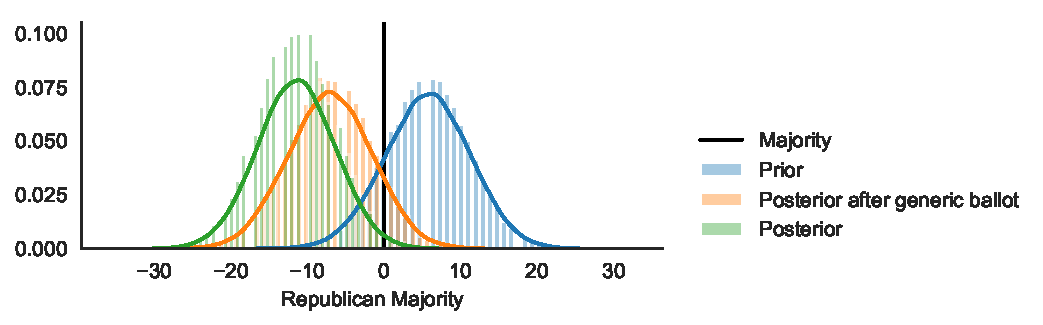
\includegraphics[width=\textwidth]{rep_seats_with_diagonal_prior.pdf}
  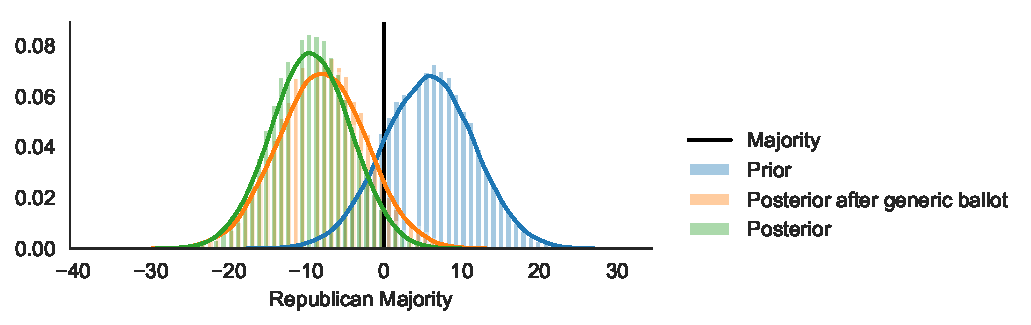
\includegraphics[width=\textwidth]{rep_seats.pdf}
  \caption{Model predictions. Top: diagonal. Bottom: unconstrained. }
  \label{fig:model}
\end{figure}


\section{Overview of prediction quality}
We plot a comparison of prediction quality between our prediction and that of FiveThirtyEight, broadly considered to be the state-of-the-art.\footnote{We take the latest prediction for each district generated by FiveThirtyEight's house model (\url{https://projects.fivethirtyeight.com/2018-midterm-election-forecast/house/}, and transform the prediction into a statistic that corresponds to \eqref{eq:def_y}.} The $R^2$ by regressing actual vote share on predicted vote share             and a constant for the diagonal model, unconstrained model, and FiveThirtyEight's            model is $0.897$, $0.893$, and $0.967$, respectively.% \Cref{tab:res} shows the number of correctly called races by model and winning party. Both \Cref{fig:quality,tab:res} show that the diagonal model performs better than the unconstrained model, and that both underperform relative to FiveThirtyEight's model. Moreover, \Cref{tab:res} shows that all three models underestimated the Democrats' performance in the midterm elections, while the diagonal outperforms unconstrained, and both of our models underperform that of FiveThirtyEight's.
\begin{figure}[tbh]
  \centering
  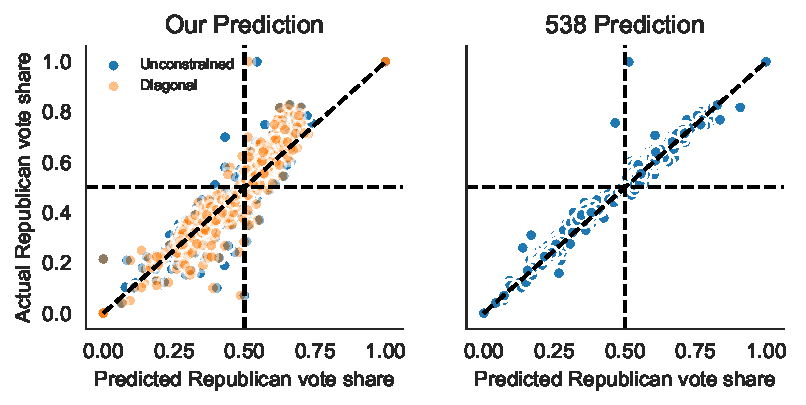
\includegraphics{prediction_quality.pdf}
  \caption{Quality of our prediction compared to that of FiveThirtyEight. The point that all predictions incurred large positive residuals is Alaska's district-at-large, where the Republican won a competitive race, yet the Republican's opponent is an Independent and not a Democrat. Thus \eqref{eq:def_y} would define the response variable being 1, even though the race is fairly competitive.}
  \label{fig:quality}
\end{figure}
\begin{table}[tb]
  \caption{Number of correctly called races for each model by winning party of each district, and number of expected seats won by Democrats compared to ground truth.}
  \label{tab:res}
  \vspace{1em}
  \centering
\begin{tabular}{lllll}
\toprule
{} & Total & Diagonal & Unconstrained &  538 \\
Winner                             &       &          &               &      \\
\midrule
Democrat                           &   240 &      216 &           211 &  226 \\
Republican                         &   195 &      190 &           187 &  193 \\
\midrule Expected Democratic Seats &   240 &      230 &           223 &  233 \\
\bottomrule
\end{tabular}

\end{table}

It is clear from \Cref{tab:res,fig:model,fig:quality} that the unconstrained model suffers from too little precision, as the correlation operator in \eqref{eq:unres_var} is extremely noisy, since the correlation is only taken over the four election years from 2010--2016. The unconstrained model was motivated by the fear that without modeling correlation of elections, the prediction model is going to be overly precise and would overlook systemic polling and modeling errors as was the case with the 2016 presidential election. However, it does seem that modeling correlation in the manner of \eqref{eq:unres_var} is not a good idea. From this point, we only consider the diagonal model. 

\begin{figure}[tbh]
  \centering
  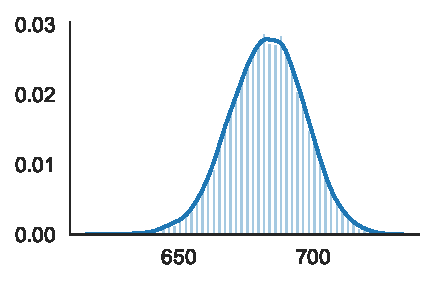
\includegraphics{likelihood_dist.pdf}
  \caption{The distribution of log likelihood over data generated from the fitted diagonal model.}
  \label{fig:likelihood}
\end{figure}

The benefit of explicit probabilistic modeling in the manner that we have done
is that we can evaluate the likelihood of the outcome that materialized. 
\Cref{fig:likelihood} displays the distribution of log-likelihood with simulated data generated according to the fitted model $\Norm(\mu,\Sigma)$. With the general intuition of hypothesis testing, we reject the model if the observed data has extremely low likelihood under the model. Evaluating the data transformed via \eqref{eq:def_y} suffers from extraordinarily low likelihood of a few observations, due to the presence of Independents (as in the caption of \Cref{fig:quality}). However, even with untransformed data, the data-likelihood is still exceptionally low compared to \Cref{fig:likelihood}:
The log-likelihood of transformed data (as in \eqref{eq:def_y}) is 41.75, while the log-likelihood of untransformed Republican vote share is 442.25.% The reason of the low likelihood seem to be that the variance of the model being too low, as $\mu$ is fairly close to the materialized outcome, by \Cref{fig:quality}. We can consider a variance inflation parameter $\sigma^2$ which maximizes the data likelihood under model $\Norm(\mu, \sigma^2 \Sigma)$. The fitted $\sigma^2$ is 4.262 for transformed data and 2.224 for untransformed data.

\section{Model selection in fitting $\mu_0$}
We examine the effect of covariate selection by running the procedure while leaving one of the covariates out, somewhat mimicking a backward stepwise model selection procedure. Since the design matrix $X$ included both linear and quadratic terms of the covariates, leaving one covariate out leaves out all its quadratic terms. We present the $R^2$ of the regression of the 2018 data on the predictions (as in \Cref{fig:quality}) in \Cref{tab:leave_out}. We see that leaving out most covariates have little effect on the prediction quality, while racial makeup, incumbency, and educational background are particularly important for prediction. Moreover, for quite a few covariates, leaving them out actually \emph{improves} fit, suggesting that the elastic net regularizer is not a panacea for overfitting---in particular, if the covariates have little predictive power, then in order for the regularizer to adequately control for overfitting, it must have a high level of shrinkage, which may result in underfitting, as the regularizer would discount variables that are highly predictive.

\begin{table}[tbh]
  \caption{Effect on fit (among competitive races) of leaving one covariate (along with all higher-power terms that involve the covariate) out; we also show the performance of certain alternative prediction functions for $\mu_0$. \texttt{full} means full model. \texttt{quadratic} means leaving out all quadratic terms. \texttt{lasso\_select} means using a cross-validated LASSO to select covariates by discarding all covariates with zero fitted coefficent and running an elastic net on the rest of the covariates. \texttt{gradient\_boost} is a gradient boosting regression tree with validation-guided early stopping. \texttt{logit} is a model where $\mu_0 = X\beta_0$ is replaced with $\mu_0 = \logit^{-1}(X\beta_0)$---we fit an elastic net on $\logit$-transformed training data to obtain $\beta_0$.}
  \label{tab:leave_out}
  \centering
  \vspace{1em}
  \begin{tabular}{lllr}
\toprule
        Variable left out / Model name &  $R^2$ &       Variable left out / Model name &  $R^2$ \\
\midrule
         \texttt{minority\_percentage} & 0.7649 &  \texttt{same\_as\_pres\_party\_rep} & 0.8215 \\
               \texttt{rep\_incumbent} & 0.8062 &             \texttt{dem\_is\_female} & 0.8217 \\
 \texttt{percent\_bachelor\_or\_above} & 0.8086 &                \texttt{dem\_percent} & 0.8230 \\
              \texttt{gradient\_boost} & 0.8138 &             \texttt{rep\_is\_female} & 0.8235 \\
               \texttt{pres\_approval} & 0.8177 &               \texttt{lasso\_select} & 0.8238 \\
             \texttt{log\_med\_income} & 0.8182 &                       \texttt{logit} & 0.8259 \\
            \texttt{rep\_to\_tot\_oct} & 0.8183 &               \texttt{kernel\_sigma} & 0.8264 \\
            \texttt{rep\_to\_tot\_nov} & 0.8211 &              \texttt{dem\_incumbent} & 0.8272 \\
                         \texttt{full} & 0.8215 &                   \texttt{quadratic} & 0.8324 \\
                                       &        &  \texttt{same\_as\_pres\_party\_dem} & 0.8402 \\
\bottomrule
\end{tabular}

\end{table}

We also experiment with a some methods to improve model selection in \Cref{tab:leave_out}, treating the data from 2018 as a validation set. In particular, the \texttt{lasso\_select} entry in \Cref{tab:leave_out} represents a two-step procedure where a first-step LASSO regression is used to select covariates and a second-step elastic net is used to further control for overfitting and shrinkage. We see that this method marginally increases quality of fit. In \texttt{quadratic}, we simply leave out all quadratic terms in $X$, and rather discouragingly, this much sparser set of covariates perform better than both the \texttt{full} and the \texttt{lasso\_select} models. 

We also investigate whether alternative methods for fitting $\mu_0 = f_\beta(X)$, for some functional form $f$ and parameters $\beta$, would have done better. We fit a gradient boosting regression tree (\texttt{gradient\_boost}) on the same input space as the original model (\texttt{full}). We hold out a validation set and use an early stopping rule---stopping when the validation error fails to improve for a number of iterations.\footnote{We tried multiple hyperparameters for the early stopping; all of them failed to generate better fit than \texttt{full}.} \texttt{gradient\_boost} does not appear to have better fit than the elastic net. We suspect that nonparametric methods like gradient boosting trees do not utilize the rich probabilistic information in the input data (the probabilistic model \eqref{eq:first} fits fairly well by inspecting a Q-Q plot; see original report for details), which results in a worse fit. This leads us to suspect that better specified probabilistic models should do better. We correct for the misspecification in \eqref{eq:first} by fitting $\beta$ on the logit-transformed space of the original data: \[
\logit(Y_\text{tr}) \sim \Norm(X_\text{tr}\beta_0, \Sigma_\text{tr}),
\]
mimicking the \emph{logit-normal model} \cite[page 283]{agresti2015foundations}---so that the Normal distribution is properly specified on data that can take values in $\R$. However, modeling in the logit space does not lend well to the simple Bayesian updating in \eqref{eq:post} without using expensive MCMC simulations, and for convenience's sake, in prediction, we modify \eqref{eq:first} to $\Norm(\logit^{-1}(X\beta_0), \Sigma_0),$ which is again a slight misspecification.\footnote{Therefore, the \texttt{logit} model in \Cref{tab:leave_out} is not strictly-speaking a logit-normal model as in \cite{agresti2015foundations}---rather an ad hoc alternative inspired by the logit-normal model in the literature.} This model, \texttt{logit}, does appear to perform slightly better than the original model \texttt{full}, but the degree of improvement is probably too small to show anything meaningful. 

\bibliographystyle{jpe}
\bibliography{main.bib}
\end{document}
